% Project - Technical Documentation
%
% Data Acquisition Technologies and Sensor Networks
% Jacobs University Bremen
% Supervisor: Prof. Dr. Fangning Hu
%
% Created on November 13, 2019
%
% Authors:
%   Ralph Florent <r.florent@jacobs-university.de>
%   Diogo Cosin <d.ayresdeoliveira@jacobs-university.de>
%   Eno Ciraku <e.ciraku@jacobs-university.de>
%
% Theory review for the documentation

% ==============================================================================
% START: Theoretical background
% ==============================================================================

\section{Theoretical Review}
\label{sec:state-of-art}

This section briefly provides information about the hardware components used in
this project. If desired, more information can be found on their respective
bibliographical references, also provided in this section.

\subsection{Arduino Mega 2560 Rev3}
\label{subsec:arduino}

The Arduino Mega 2560 Rev3, showed in Figure \ref{fig:arduino}, is a microcontroller based on the the Atmel's 
microcontroller ATmega2560. In this subsection, we limitate ourselves to the 
ArduinoMega 2560 Rev3. However, general and technical details about the
microcontroller ATmega2560 can be found in \cite{arduinospecs}.

\begin{figure}[h!]
    \centering
    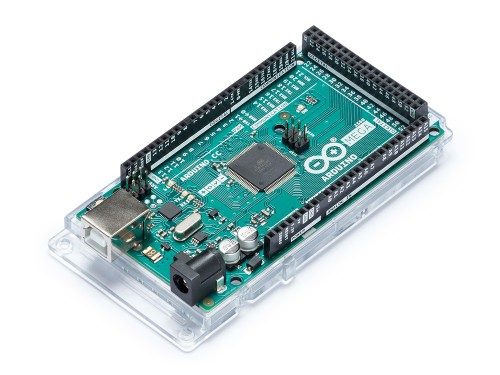
\includegraphics[scale=0.45]{arduino.jpg}
    \caption{An Arduino Mega Rev3 unity.}
    \label{fig:arduino}
\end{figure}

A microcontroller is an electronic device and a small computer placed on a single
metal-oxide-semiconductor (MOS) integrated circuit. It contains at least one
Central Processing Unit (CPU), memory, and input/output peripherals which
interface in different voltage levels, typically 3.3V and 5V. Program memory is
also included in this type of device. This way, developers can adapt the device logically according to the desired application. They are normally deployed in
embedded systems such as automobile engine control systems, implantable medical
devices, remote controls, office machines, among others. With the new Internet of Things
(IoT) trend, these devices act in data collection, sensing, and actuating
components in the physical world \cite{microcontroller}.

Besides the microcontroller itself, the Arduino Mega 2560 Rev3 also contains 54 
digital input/output pins, 16 analog inputs, 4 UARTs, a 16 MHz crystal
oscillator, a USB connection, a power jack, an ICSP header, and a reset button. 
Through external shields, the technical capabilities may be extended for
different purposes, such as Bluetooth, ZigBee, Wi-Fi, and GPS connections, among
others \cite{arduinospecs}.

Through its Integrated Development Environment (IDE), developers can program this
microcontroller according to the required application. The Arduino programming
language is a collection of C and C++ functions called as specified by the
developers. Behind the hoods, these functions are directed to a C/C++ compiler.
Nevertheless, it worths mentioning that developers can also use different software to 
program Arduino, however, some extra steps are required \cite{arduinofaq}.

\subsection{Elegoo 4-Channel Relay}

The Elegoo's 4-channel relay GE-EL-SM-006, showed in Figure \ref{fig:relay}, is
a set of 4 relays 5V active low. It also provides 4 Ligh-emitting diodes (LEDs)
for verification of the relays' status.

\begin{figure}[h!]
    \centering
    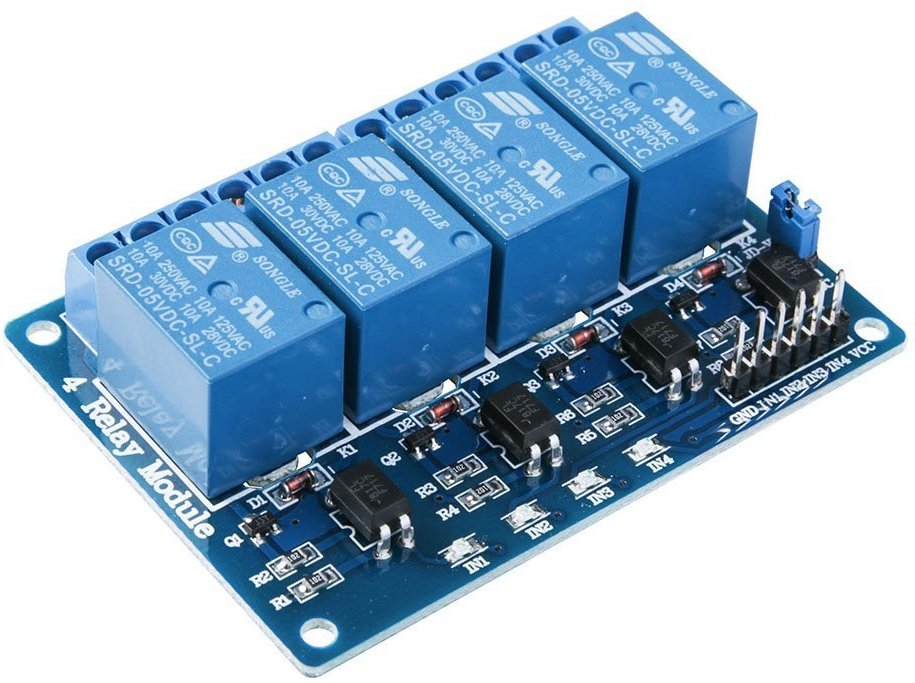
\includegraphics[scale=0.15]{4-channel_relay.jpg}
    \caption{The Elegoo's 4-channel relay GE-EL-SM-006.}
    \label{fig:relay}
\end{figure}

A relay is an electrical switch that controls its status (open or closed) according
to the input signal. In its traditional form, a magnetic field is created to attract
a coil and consequently close the contact, hence the switch behavior. In
addition, other operating principles have been created, as in solid-state relays
that use semiconductor features for control. These devices are commonly applied
as electrical switches, as in the project presented in this report, but also 
protective systems \cite{relay}.

This module also allows the interface with different controllers, among them the Arduino
(briefly introduced in the Subsection \ref{subsec:arduino}). These
controllers can be then particularly programmed to command the 4-Channel relay
states.

\subsection{Espressif ESP8266EX}

The Espressif's ESP8266EX, showed in Figure \ref{fig:ESP8266EX}, is a System on a
Chip (SoC), an integrated circuit, which offers Wi-Fi networking capability as
well as microcontroller capabilities. It can be deployed in standalone
applications, given that it gives CPU, programmable Random-access memory (RAM), and Read-only memory (ROM), that is, capabilities that a microcontroller
provides. Not only that, but the ESP8266EX can also be employed in applications as
the slave to a host microcontroller. For example, the device can be applied to
any microcontroller as a Wi-Fi adaptor, as designed in this report's project \cite{wifi}.

\begin{figure}[h!]
    \centering
    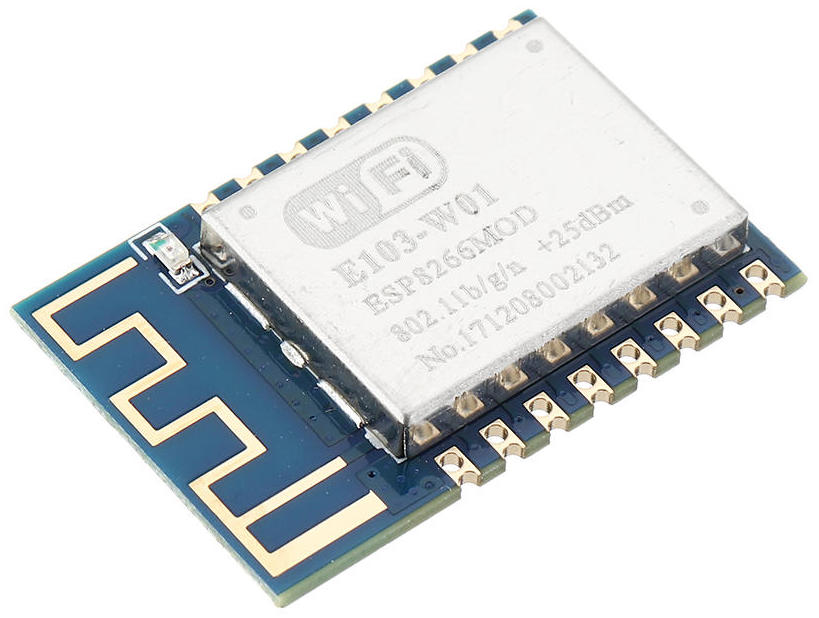
\includegraphics[scale=0.15]{ESP8266EX.jpg}
    \caption{The Espressif's ESP8266EX.}
    \label{fig:ESP8266EX}
\end{figure}

Some key capabilities of the Espressif's ESP8266EX follows \cite{wifi}:

\begin{itemize}
    \item \textbf{Wi-Fi support:} 802.11 b/g/n, 802.11 n support (2.4 GHz), up to 72.2 Mbps;
    \item \textbf{CPU:} Tensilica L106 32-bit Reduced instruction set computer (RISC)
    processor;
    \item \textbf{Memory:} includes memory controller and memory units including
    SRAM and ROM;
    \item \textbf{External flash:} external SPI flash to store user programs,
    supporting up to 16MB;
    \item \textbf{Clock:} clock generated from internal crystal oscillator and
    extenal crystal;
    \item \textbf{General Purpose Input/Output Interface (GPIO):} 17 GPIO pins
    which can be customized according to the program logic;
    \item \textbf{I2C:} interface with other microcontrollers and other
    peripheral equipments performed via software programming.
\end{itemize}

Others technical features of the ESP8266EX include: Universal Asynchronous
Receiver Transmitter (UART), Pulse-Width Modulation (PWM), Infrared (IR) Remote
Control, Analog-to-Digital Converter (ADC) \cite{wifi}.

% ==============================================================================
% END: Theoretical background
% ==============================================================================